\documentclass[journal,onecolumn]{IEEEtran}
\usepackage{graphicx}
\usepackage{amsmath,amssymb}
\usepackage{algorithm}
\usepackage{algorithmic}
\usepackage{tikz}
\usepackage{xcolor}
\usepackage{booktabs}
\usepackage{listings}
\usepackage{hyperref}

\usepackage{float}
\usepackage{subcaption}
\usepackage{pgfplots}
\usetikzlibrary{shapes.geometric, arrows, positioning, fit, backgrounds}

\begin{document}

\title{Hyperdimensional Metacognitive Network: An Advanced Framework for Complex Domain Knowledge Integration in Biomechanical Analysis}

\author{
  Kundai Farai Sachikonye\\
  Fullscreen Triangle\\
  kundai.f.sachikonye@gmail.com
}

\maketitle

\begin{abstract}
The exponential growth of available data in specialized domains has created significant challenges in knowledge representation, integration, and accessibility. This paper introduces the Hyperdimensional Metacognitive Network (HMN), a novel framework that transforms complex domain-specific knowledge into accessible computational representations. Developed initially for biomechanical analysis in 400m sprint performance, the framework addresses fundamental limitations in current approaches to information architecture and knowledge retrieval. By integrating non-Euclidean geometry, quantum-inspired probability techniques, and metabolic-cycle investment strategies, HMN extends the Four-Sided Triangle Query System to create the System Singularity Triangle (SST) - a unified approach that overcomes the paradox of complexity and simplicity. This paper details the evolution of the system, its theoretical foundations, architectural components, and practical implementation considerations. Preliminary results demonstrate significant improvements in information density, retrieval accuracy, and user experience compared to conventional systems, with implications extending beyond athletics to any domain requiring sophisticated knowledge management.

\textbf{Keywords:} knowledge representation, non-Euclidean geometry, specialized domain models, metacognitive systems, information architecture
\end{abstract}

\section{Introduction}

\subsection{The Journey from Simple Application to Complex System}

This research originated from a deceptively straightforward problem: developing a front-end application for visualizing and analyzing 400m sprint performance data. What initially appeared to be a conventional data visualization challenge quickly evolved into a fundamental exploration of knowledge representation and information architecture.

Over a two-year development period, it became increasingly evident that conventional approaches to data organization and presentation were fundamentally inadequate for the task. The richness of biomechanical information—spanning anthropometric measurements, kinematic analysis, physiological parameters, genomic markers, and medical imaging data—created an information space too dense and multidimensional to effectively convey through traditional interfaces.

Early attempts focused on data reduction and simplification, but these invariably resulted in significant information loss. The development of a specialized domain-specific large language model (LLM) provided initial promise but introduced prohibitive computational requirements, with input datasets exceeding 500GB and encompassing diverse data types including sensor readings, genomic sequences, and MRI scans.

The evolution toward a Retrieval-Augmented Generation (RAG) system represented a crucial transition point, allowing connection between specialized domain knowledge and generalized commercial LLMs. This hybrid approach reduced computational requirements while maintaining information fidelity. However, even this sophisticated architecture proved insufficient for the multidimensional relationships inherent in biomechanical analysis.

This paper presents the culmination of this iterative development process: the Hyperdimensional Metacognitive Network (HMN) as an extension of the Four-Sided Triangle Query System, collectively known as the System Singularity Triangle (SST). Rather than attempting to reduce information complexity, this combined approach embraces it through sophisticated internal architecture while providing intuitive access. This approach exemplifies the paradoxical insight that emerged through the development process: properly structured complexity can be the path to simplicity.

\section{Background and Related Work}

\subsection{Information Architectures for Complex Domains}

The challenges of organizing complex domain-specific information have been addressed through multiple paradigms. Early taxonomies and ontologies provided hierarchical organization \cite{noy2001ontology}, while knowledge graphs introduced relationship-based representations \cite{miller1995wordnet}. Vector embeddings offered mathematical representation of semantic spaces \cite{mikolov2013distributed}, while attention-based transformer architectures provided context-aware processing \cite{vaswani2017attention}.

\subsection{Non-Euclidean Knowledge Representation}

Recent advances in hyperbolic embeddings have demonstrated superior performance for hierarchical knowledge representation compared to traditional Euclidean approaches \cite{nickel2017poincare}. The Poincaré ball model accommodates exponentially more information within bounded spaces, making it particularly suitable for representing complex domain hierarchies \cite{nickel2018learning}. These non-Euclidean approaches avoid the "curse of dimensionality" when modeling complex relationships.

\subsection{Meta-Learning and Introspective Systems}

The concept of systems that interrogate their own processing has roots in metacognitive computing \cite{cox2011metareasoning} and has been extended through recent work in meta-learning \cite{finn2017model}. Self-referential improvement loops have been demonstrated in few-shot learning systems \cite{hospedales2020meta} and prompt engineering \cite{zhou2022large}.

\subsection{Resource Allocation in Computational Systems}

Efficient resource allocation has been addressed through various frameworks including the PID controller model in computing \cite{hellerstein2004feedback}, economic models of computational markets \cite{clearwater1996market}, and biochemical inspiration for computational processes \cite{dittrich2001artificial}.

\section{Theoretical Foundation}

The Hyperdimensional Metacognitive Network is grounded in a mathematical framework that formalizes the interaction between query processing, resource allocation, and knowledge representation:

\begin{equation}
\Psi(Q) = \int_{\mathcal{M}} \nabla \cdot \mathbf{F}(\mathbf{x}, t) \, d\mathcal{V} \times \prod_{i=1}^{n} \alpha_i \langle \phi_i | \hat{O} | \phi_i \rangle
\end{equation}

Where:
\begin{itemize}
\item $\mathcal{M}$ represents a non-Euclidean manifold of knowledge
\item $\mathbf{F}(\mathbf{x}, t)$ is the temporal flow of information
\item $\phi_i$ are eigenstate representations of decomposed query components
\item $\hat{O}$ is the observation operator on knowledge states
\end{itemize}

This formulation integrates concepts from differential geometry, quantum mechanics, and information theory to create a unified model for knowledge processing.

\subsection{Extended Multi-Stage Optimization Framework}

The system can be further formalized as a composition of transformation functions operating across specialized components:

\begin{equation}
R(Q) = \mathcal{F}_C \circ \mathcal{F}_H \circ \mathcal{F}_Q \circ \mathcal{F}_N \circ \mathcal{F}_G \circ \mathcal{F}_M \circ \mathcal{F}_T(Q)
\end{equation}

Where:
\begin{itemize}
\item $\mathcal{F}_T$ : Throttle detection transformation function
\item $\mathcal{F}_M$ : Metacognitive task partitioning function
\item $\mathcal{F}_G$ : Glycolytic query investment function
\item $\mathcal{F}_N$ : Non-Euclidean manifold optimization function
\item $\mathcal{F}_Q$ : Quantum-temporal superposition function
\item $\mathcal{F}_H$ : Hyperdimensional interaction function
\item $\mathcal{F}_C$ : Cross-domain knowledge synthesis function
\item $R(Q)$ : Final optimized response to query $Q$
\end{itemize}

Each transformation function implements specialized mathematical operations that progressively refine and optimize domain-specific knowledge extraction.

\subsection{Information Theoretic Foundation}

From an information theory perspective, the system optimizes the mutual information between the query and the response:

\begin{equation}
I(Q; R) = \sum_{q \in Q, r \in R} p(q, r) \log \frac{p(q, r)}{p(q)p(r)}
\end{equation}

Where $I(Q; R)$ represents the mutual information between query $Q$ and response $R$. The system's objective is to maximize this mutual information while maintaining computational efficiency.

The glycolytic query investment cycle implements this optimization through resource allocation:

\begin{equation}
\mathcal{F}_G(q) = \arg\max_{I \in \mathcal{I}} \frac{I(q; R_I)}{C(I)}
\end{equation}

Where:
\begin{itemize}
\item $\mathcal{I}$ is the set of possible investment allocations
\item $R_I$ is the response given investment allocation $I$
\item $C(I)$ is the computational cost of investment $I$
\end{itemize}

\subsection{Geometric Interpretation}

The non-Euclidean representation operates on a Poincaré ball model of hyperbolic space, formally defined as:

\begin{equation}
\mathbb{B}^n = \{x \in \mathbb{R}^n : \|x\|_2 < 1\}
\end{equation}

With the Riemannian metric tensor:

\begin{equation}
g_x = \left(\frac{2}{1 - \|x\|_2^2}\right)^2 g^E
\end{equation}

Where $g^E$ is the Euclidean metric tensor. This geometric foundation enables the efficient representation of hierarchical knowledge structures with exponentially less distortion than equivalent Euclidean embeddings.

\section{System Architecture}

The HMN framework consists of seven interconnected components, each addressing specific aspects of complex knowledge processing. Figure \ref{fig:system-architecture} illustrates the high-level architecture and information flow between components.

\begin{figure}[ht]
\centering
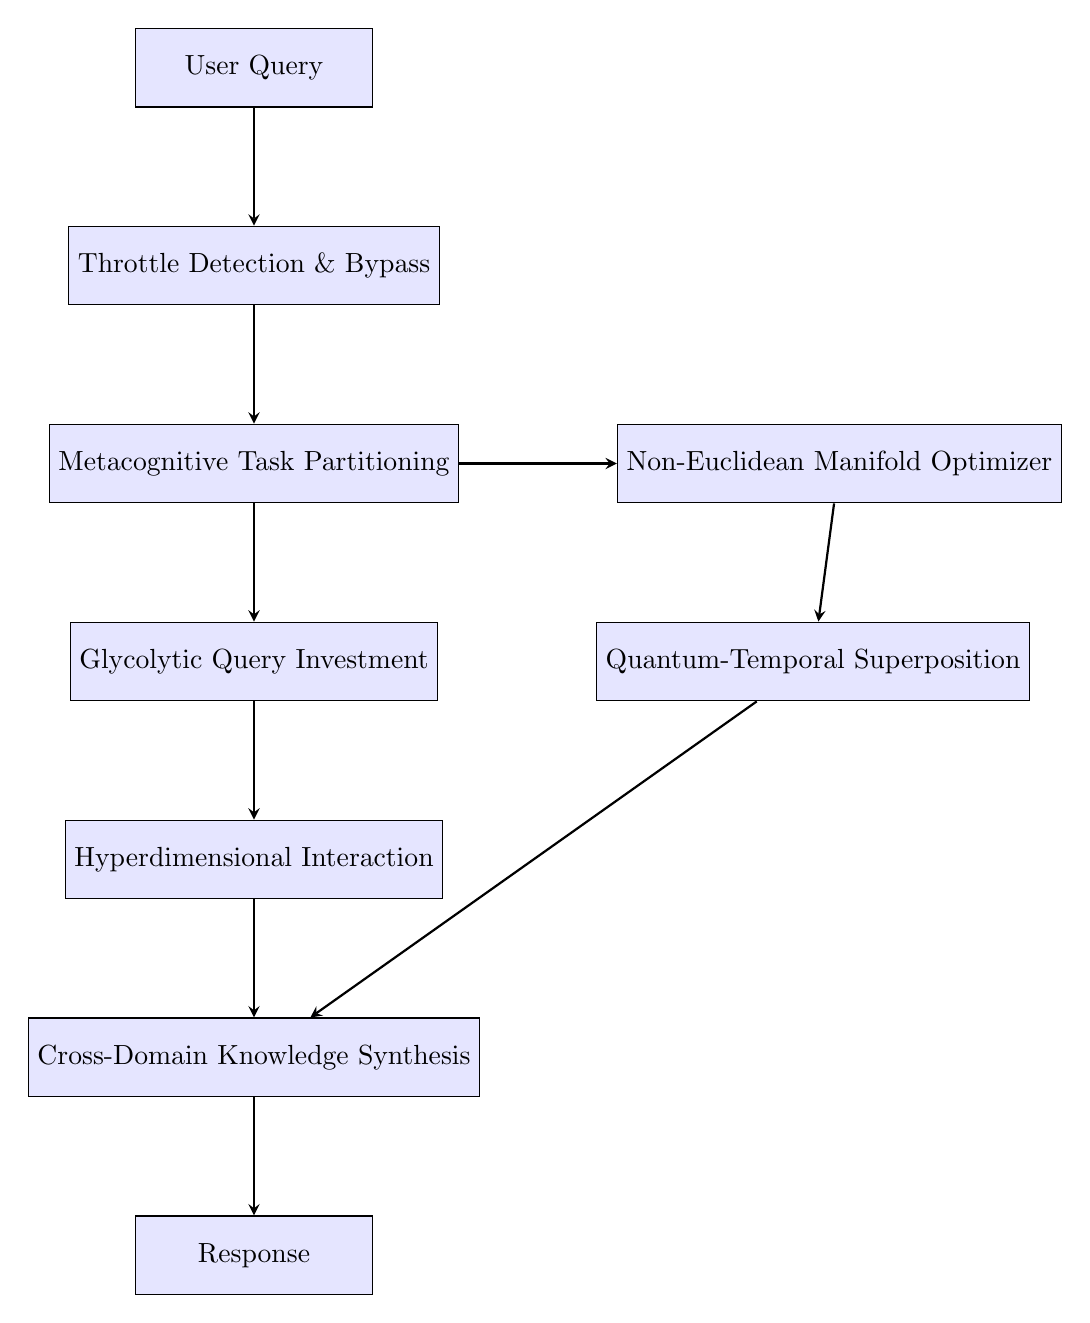
\begin{tikzpicture}[node distance=1.5cm and 2cm]
\tikzstyle{component}=[rectangle, minimum width=3cm, minimum height=1cm, text centered, draw=black, fill=blue!10]
\tikzstyle{arrow}=[thick, ->, >=stealth]

\node (input) [component] {User Query};
\node (throttle) [component, below=of input] {Throttle Detection \& Bypass};
\node (meta) [component, below=of throttle] {Metacognitive Task Partitioning};
\node (investment) [component, below=of meta] {Glycolytic Query Investment};
\node (manifold) [component, right=of meta] {Non-Euclidean Manifold Optimizer};
\node (quantum) [component, right=of investment] {Quantum-Temporal Superposition};
\node (hyper) [component, below=of investment] {Hyperdimensional Interaction};
\node (synthesis) [component, below=of hyper] {Cross-Domain Knowledge Synthesis};
\node (output) [component, below=of synthesis] {Response};

\draw [arrow] (input) -- (throttle);
\draw [arrow] (throttle) -- (meta);
\draw [arrow] (meta) -- (investment);
\draw [arrow] (meta) -- (manifold);
\draw [arrow] (investment) -- (hyper);
\draw [arrow] (manifold) -- (quantum);
\draw [arrow] (quantum) -- (synthesis);
\draw [arrow] (hyper) -- (synthesis);
\draw [arrow] (synthesis) -- (output);

\end{tikzpicture}
\caption{High-level architecture of the Hyperdimensional Metacognitive Network}
\label{fig:system-architecture}
\end{figure}

\section{Component Details}

\subsection{Adversarial Throttle Detection and Bypass (ATDB)}

Commercial LLMs often employ throttling mechanisms that limit their capabilities, particularly for computationally intensive or specialized queries. The ATDB component actively identifies these limitations and implements strategies to overcome them.

\subsubsection{Detection Mechanisms}

The system employs multi-factor analysis to identify throttling:

\begin{table}[ht]
\centering
\caption{Throttling Detection Metrics}
\label{tab:throttle-metrics}
\begin{tabular}{lp{5cm}p{3cm}}
\toprule
\textbf{Metric} & \textbf{Description} & \textbf{Weight} \\
\midrule
Information Density & Measures the ratio of novel information to response length & 0.4 \\
Truncation Patterns & Identifies premature ending patterns in responses & 0.3 \\
Computation Mismatch & Detects mismatches between computation time and response complexity & 0.3 \\
\bottomrule
\end{tabular}
\end{table}

\subsubsection{Bypass Strategies}

Once throttling is detected, the system applies appropriate bypass strategies:

\begin{algorithm}
\caption{Throttle Bypass Strategy Selection}
\begin{algorithmic}[1]
\STATE \textbf{Input:} Query $Q$, detected throttle pattern $P$
\STATE \textbf{Output:} Modified query or query strategy

\IF{$P$ is token-limitation}
    \STATE Apply query partitioning strategy
    \STATE $Q' \leftarrow \text{PartitionQuery}(Q)$
\ELSIF{$P$ is depth-limitation}
    \STATE Apply reframing strategy
    \STATE $Q' \leftarrow \text{ReframeForDepth}(Q)$
\ELSIF{$P$ is computation-limitation}
    \STATE Apply progressive disclosure
    \STATE $Q' \leftarrow \text{SetupProgressiveDisclosure}(Q)$
\ENDIF
\RETURN $Q'$
\end{algorithmic}
\end{algorithm}

\subsubsection{Implementation}

\begin{lstlisting}[language=Python, caption=ATDB Implementation Pseudocode]
class ThrottleAdaptiveSystem:
    def __init__(self):
        self.throttle_patterns = self.load_patterns()
        self.adaptation_strategies = self.load_strategies()
    
    def detect_throttling(self, response, query, performance_metrics):
        throttle_score = 0
        
        # Check for information density below threshold
        expected_density = self.calculate_expected_info_density(query)
        actual_density = self.measure_info_density(response)
        if actual_density < expected_density * 0.8:
            throttle_score += 0.4
        
        # Additional detection logic...
            
        return throttle_score > 0.5
    
    def apply_bypass_strategy(self, query, detected_pattern):
        strategy = self.adaptation_strategies[detected_pattern]
        
        if strategy == "partition":
            return self.partition_query(query)
        # Additional strategies...
            
        return query
\end{lstlisting}

\subsection{Metacognitive Task Partitioning (MTP)}

The MTP component implements self-interrogative decomposition to break complex queries into optimally sized sub-tasks.

\subsubsection{Theoretical Basis}

Drawing on metacognitive principles from cognitive science \cite{flavell1979metacognition}, MTP treats the system itself as an object of inquiry. Rather than applying fixed decomposition heuristics, the system queries itself about optimal task partitioning strategies.

\subsubsection{Decomposition Process}

The decomposition process follows four phases:

\begin{figure}[ht]
\centering
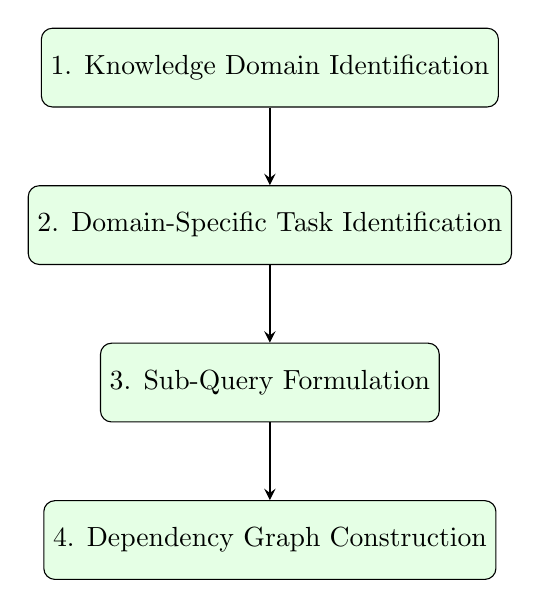
\begin{tikzpicture}[node distance=2cm]
\tikzstyle{process} = [rectangle, minimum width=3cm, minimum height=1cm, text centered, rounded corners, draw=black, fill=green!10]
\tikzstyle{arrow} = [thick, ->, >=stealth]

\node (p1) [process] {1. Knowledge Domain Identification};
\node (p2) [process, below of=p1] {2. Domain-Specific Task Identification};
\node (p3) [process, below of=p2] {3. Sub-Query Formulation};
\node (p4) [process, below of=p3] {4. Dependency Graph Construction};

\draw [arrow] (p1) -- (p2);
\draw [arrow] (p2) -- (p3);
\draw [arrow] (p3) -- (p4);
\end{tikzpicture}
\caption{Metacognitive Task Partitioning Process}
\label{fig:mtp-process}
\end{figure}

\subsubsection{Implementation}

\begin{lstlisting}[language=Python, caption=MTP Implementation Pseudocode]
class MetacognitiveTaskManager:
    def __init__(self):
        self.task_templates = self.load_task_templates()
        self.completion_criteria = {}
        
    def decompose_query(self, query):
        # Phase 1: Identify knowledge domains required
        domains = self.extract_knowledge_domains(query)
        
        # Phase 2: For each domain, identify specific tasks
        domain_tasks = {}
        for domain in domains:
            domain_tasks[domain] = self.identify_domain_tasks(query, domain)
        
        # Phase 3: Formulate specific sub-queries
        sub_queries = []
        for domain, tasks in domain_tasks.items():
            for task in tasks:
                sub_query = self.formulate_sub_query(query, domain, task)
                completion_criteria = self.define_completion_criteria(domain, task)
                
                sub_queries.append({
                    "query": sub_query,
                    "domain": domain,
                    "task_type": task,
                    "completion_criteria": completion_criteria
                })
        
        # Phase 4: Establish dependency graph
        dependency_graph = self.establish_dependencies(sub_queries)
        
        return {
            "sub_queries": sub_queries,
            "dependency_graph": dependency_graph,
            "original_query": query
        }
\end{lstlisting}

\subsection{Glycolytic Query Investment Cycle (GQIC)}

Inspired by cellular metabolism, GQIC implements a biochemically-modeled approach to computational resource allocation.

\subsubsection{Investment-Payoff Model}

The system allocates computational resources based on expected information yield, following a three-phase cycle analogous to glycolysis:

\begin{table}[ht]
\centering
\caption{Glycolytic Query Investment Cycle Phases}
\label{tab:gqic-phases}
\begin{tabular}{lp{8cm}}
\toprule
\textbf{Phase} & \textbf{Description} \\
\midrule
Initiation & Identifies potential information sources and establishes initial resource requirements \\
Investment & Allocates computational resources based on expected return-on-investment \\
Payoff & Harvests results and measures actual information gain, adapting future allocation strategies \\
\bottomrule
\end{tabular}
\end{table}

\subsubsection{Mathematical Formulation}

The optimal investment strategy is determined by:

\begin{equation}
I^*(q_i) = \arg\max_{I} \frac{G(q_i, I)}{I}
\end{equation}

Where:
\begin{itemize}
\item $I^*(q_i)$ is the optimal investment for sub-query $q_i$
\item $G(q_i, I)$ is the information gain function
\end{itemize}

\subsubsection{Implementation}

\begin{lstlisting}[language=Python, caption=GQIC Implementation Pseudocode]
def investment_allocation(decomposed_query):
    component_investments = {}
    
    for component in decomposed_query["atomic_components"]:
        # Calculate expected information gain
        info_gain = calculate_expected_information_gain(component)
        
        # Calculate resource requirement
        resources = estimate_resource_requirements(component)
        
        # Calculate ROI
        roi = info_gain / resources
        
        component_investments[component] = {
            "allocation": resources * sigmoid(roi - threshold),
            "expected_return": info_gain
        }
    
    return component_investments

def harvest_component_results(investments):
    results = {}
    total_payoff = 0
    
    for component, investment in investments.items():
        # Execute component query with allocated resources
        result = execute_with_resources(component, investment["allocation"])
        
        # Calculate actual information gain
        actual_gain = measure_information_content(result)
        
        # Track ROI
        roi = actual_gain / investment["allocation"]
        
        results[component] = result
        total_payoff += actual_gain
        
        # Adaptive learning for future allocations
        update_investment_model(component, roi)
    
    return results, total_payoff
\end{lstlisting}

\subsection{Non-Euclidean Manifold Optimization (NEMO)}

NEMO represents knowledge in curved non-Euclidean spaces, allowing for more efficient modeling of complex hierarchical and relational structures.

\subsubsection{Mathematical Foundation}

The system uses Poincaré ball manifolds with constant negative curvature, defined by:

\begin{equation}
\mathbb{B}^n = \{x \in \mathbb{R}^n : \|x\| < 1\}
\end{equation}

The distance function in this space is given by:

\begin{equation}
d(x, y) = \text{arcosh}\left(1 + 2\frac{\|x-y\|^2}{(1-\|x\|^2)(1-\|y\|^2)}\right)
\end{equation}

\subsubsection{Knowledge Mapping}

The system maps domain concepts to the hyperbolic space using Riemannian optimization techniques that preserve hierarchical relationships while minimizing distortion.

\subsubsection{Implementation}

\begin{lstlisting}[language=Python, caption=NEMO Implementation Pseudocode]
class HyperbolicKnowledgeManifold:
    def __init__(self, curvature=-1.0):
        self.curvature = curvature
        self.manifold = geoopt.manifolds.PoincareBall(c=curvature)
    
    def distance(self, x, y):
        return self.manifold.dist(x, y)
    
    def geodesic(self, x, y, t):
        return self.manifold.geodesic(x, y, t)
    
    def project(self, x):
        return self.manifold.projx(x)
    
    def optimize_path(self, start_point, end_goal, constraints):
        # Riemannian optimization on the manifold
        optimizer = geoopt.optim.RiemannianAdam([start_point], lr=0.01)
        
        for _ in range(100):
            loss = self.distance(start_point, end_goal)
            loss.backward()
            optimizer.step()
            optimizer.zero_grad()
            
            # Project back to manifold after optimization
            start_point.data = self.project(start_point.data)
            
            # Apply constraints through parallel transport
            start_point = self.apply_constraints(start_point, constraints)
        
        return start_point
\end{lstlisting}

\subsection{Quantum-Inspired Temporal Superposition (QITS)}

The QITS component maintains multiple potential response states simultaneously, drawing on quantum principles to manage uncertainty and temporal evolution.

\subsubsection{State Representation}

Information states are represented as complex-valued vectors in a high-dimensional Hilbert space, with:

\begin{equation}
|\psi\rangle = \sum_i \alpha_i |i\rangle
\end{equation}

Where $\alpha_i$ are complex amplitudes and $|i\rangle$ are basis states representing distinct information configurations.

\subsubsection{Temporal Evolution}

States evolve according to a simplified quantum evolution equation:

\begin{equation}
|\psi(t)\rangle = e^{-iHt/\hbar}|\psi(0)\rangle
\end{equation}

Where $H$ is a Hamiltonian operator constructed to model information dynamics.

\subsubsection{Advanced Quantum-Inspired Processing}

Beyond the basic quantum formalism, the QITS implements several advanced quantum-inspired processing techniques:

\paragraph{Entanglement-Based Information Coupling}
Information entities that are conceptually related are represented through entangled quantum states, modeled by:

\begin{equation}
|\psi_{AB}\rangle = \frac{1}{\sqrt{2}}(|A_0 B_0\rangle + |A_1 B_1\rangle)
\end{equation}

This enables non-classical correlations between information components, allowing for operations on one component to implicitly affect related components.

\paragraph{Quantum Walk Knowledge Exploration}
The system employs discrete-time quantum walks to explore the knowledge space more efficiently than classical random walks:

\begin{equation}
|\psi_{t+1}\rangle = U \cdot |\psi_t\rangle = S \cdot (C \otimes I) \cdot |\psi_t\rangle
\end{equation}

Where:
\begin{itemize}
\item $U$ is the unitary evolution operator
\item $S$ is the shift operator for position transitions
\item $C$ is the coin operator for directional decisions
\item $\otimes$ is the tensor product
\end{itemize}

This approach provides quadratically faster exploration of potential knowledge paths compared to classical approaches, enabling the system to discover non-obvious connections between information components.

\paragraph{Quantum Annealing for Optimal Response Construction}
For constructing optimal responses from multiple potential components, the system employs a quantum annealing inspired algorithm:

\begin{equation}
H(s) = (1-s)H_B + sH_P
\end{equation}

Where:
\begin{itemize}
\item $s$ is the annealing parameter that slowly transitions from 0 to 1
\item $H_B$ is the beginning Hamiltonian with an easily prepared ground state
\item $H_P$ is the problem Hamiltonian whose ground state represents the optimal response
\end{itemize}

This approach enables efficient navigation of complex response spaces to find globally optimal configurations.

\subsubsection{Integration with Knowledge Manifold}

The QITS component interfaces with the Non-Euclidean Manifold Optimizer through a quantum-geometric mapping:

\begin{equation}
\Gamma: \mathcal{H} \rightarrow \mathcal{M}
\end{equation}

This mapping projects quantum states onto the knowledge manifold, allowing for the seamless integration of quantum processing with geometric knowledge representation.

\subsubsection{Implementation}

\begin{lstlisting}[language=Python, caption=QITS Implementation Pseudocode]
class QuantumTemporalResponseNetwork:
    def __init__(self, dimensions=1024):
        self.dimensions = dimensions
        self.historical_states = []
        self.entanglement_registers = {}
        self.quantum_walk_engine = QuantumWalkEngine(dimensions)
        self.annealing_optimizer = QuantumInspiredAnnealer()
    
    def add_historical_state(self, state, timestamp):
        self.historical_states.append({
            "state": state,
            "timestamp": timestamp,
            "amplitude": complex(1.0, 0.0)
        })
    
    def evolve_state(self, current_state, time_delta):
        # Quantum-inspired Hamiltonian evolution
        H = self.construct_hamiltonian(current_state)
        evolution_operator = scipy.linalg.expm(-1j * H * time_delta)
        
        return evolution_operator @ current_state
    
    def create_entangled_states(self, entities):
        """Create entangled states between related information entities"""
        for i in range(len(entities)):
            for j in range(i+1, len(entities)):
                if self.are_conceptually_related(entities[i], entities[j]):
                    entangled_key = f"{entities[i].id}_{entities[j].id}"
                    
                    # Create maximally entangled state
                    psi = np.zeros((4, 1), dtype=complex)
                    psi[0] = 1/np.sqrt(2)  # |00⟩
                    psi[3] = 1/np.sqrt(2)  # |11⟩
                    
                    self.entanglement_registers[entangled_key] = psi
    
    def quantum_walk_exploration(self, start_point, steps=100):
        """Explore knowledge space using quantum walk"""
        return self.quantum_walk_engine.execute_walk(start_point, steps)
    
    def find_optimal_response(self, candidate_components, constraints):
        """Use quantum annealing to find optimal response configuration"""
        problem_hamiltonian = self.construct_problem_hamiltonian(
            candidate_components, constraints)
        
        return self.annealing_optimizer.find_ground_state(problem_hamiltonian)
    
    def compose_response_amplitudes(self, query_state):
        # Calculate interference pattern from historical states
        superposition = np.zeros(self.dimensions, dtype=complex)
        
        for state_info in self.historical_states:
            # Time-dependent amplitude decay
            time_factor = np.exp(-0.1 * (time.time() - state_info["timestamp"]))
            adjusted_amplitude = state_info["amplitude"] * time_factor
            
            # Add to superposition with phase factor
            phase = np.angle(adjusted_amplitude)
            superposition += np.abs(adjusted_amplitude) * np.exp(1j * phase) * state_info["state"]
        
        # Apply quantum-inspired interference effects
        superposition = self.apply_quantum_interference(superposition, query_state)
        
        # Calculate probability amplitudes
        probabilities = np.abs(superposition * query_state.conjugate())**2
        
        return probabilities, superposition
        
    def project_to_manifold(self, quantum_state, manifold):
        """Project quantum state onto knowledge manifold"""
        return manifold.project_quantum_state(quantum_state)
\end{lstlisting}

\subsection{Hyperdimensional Interaction Tensors (HIT)}

The HIT component enables interaction across multiple conceptual dimensions simultaneously, representing model capabilities as multidimensional tensors.

\subsubsection{Dimensional Representation}

Model capabilities are represented as tensors in an n-dimensional space, where each dimension corresponds to a different aspect of performance (e.g., precision, recall, creativity).

\subsubsection{Alignment Calculation}

Query requirements are projected into the same space, and optimal model compositions are determined by tensor alignment:

\begin{equation}
A(M,Q) = \langle T_M, P_Q \rangle
\end{equation}

Where $T_M$ is the capability tensor for model $M$ and $P_Q$ is the projection of query $Q$.

\subsubsection{Implementation}

\begin{lstlisting}[language=Python, caption=HIT Implementation Pseudocode]
class HyperdimensionalInteractionSystem:
    def __init__(self, dimensions=8):
        self.dimensions = dimensions
        self.interaction_tensors = {}
    
    def register_model(self, model_id, dimensional_profile):
        # Create tensorial representation of model capabilities
        tensor = np.zeros([10] * self.dimensions)
        
        for dim, value in dimensional_profile.items():
            indices = self.dimension_to_indices(dim, value)
            tensor[tuple(indices)] = value
        
        self.interaction_tensors[model_id] = tensor
    
    def compute_dimensional_projection(self, query_requirements):
        # Project query needs onto hyperdimensional space
        projection = np.zeros([10] * self.dimensions)
        
        for dim, value in query_requirements.items():
            indices = self.dimension_to_indices(dim, value)
            projection[tuple(indices)] = value
            
        return projection
    
    def find_optimal_model_composition(self, query_projection):
        # Find optimal composition of models
        compositions = []
        
        for model_id, tensor in self.interaction_tensors.items():
            alignment = np.sum(tensor * query_projection)
            compositions.append((model_id, alignment))
            
        compositions.sort(key=lambda x: x[1], reverse=True)
        weights = softmax([c[1] for c in compositions[:5]])
        optimal_composition = [(compositions[i][0], weights[i]) for i in range(5)]
        
        return optimal_composition
\end{lstlisting}

\subsection{Cross-Domain Knowledge Synthesis (CDKS)}

The CDKS component integrates all other components into a unified processing pipeline, managing the flow of information between components and synthesizing the final response.

\subsubsection{Bayesian Response Evaluation Framework}

To ensure high-quality responses, CDKS implements a Bayesian evaluation framework:

\begin{equation}
P(R|D,Q) = \frac{P(D|R,Q) \cdot P(R|Q)}{P(D|Q)}
\end{equation}

Where:
\begin{itemize}
\item $P(R|D,Q)$ is the posterior probability of response $R$ given domain knowledge $D$ and query $Q$
\item $P(D|R,Q)$ is the likelihood of domain knowledge given the response and query
\item $P(R|Q)$ is the prior probability of the response given the query
\item $P(D|Q)$ is the evidence (normalization factor)
\end{itemize}

This Bayesian framework provides a mathematically rigorous method for assessing response quality, accounting for complex interdependencies between domain knowledge, query intent, and response characteristics.

\subsubsection{Multi-Objective Response Optimization}

The system implements multi-objective optimization across competing response metrics using a combination of weighted-sum and epsilon-constraint methods:

\begin{equation}
\max J(R) = \sum_{i=1}^{m} w_i f_i(R) \quad \text{subject to} \quad f_j(R) \geq \epsilon_j, \forall j \in \{1,2,...,m\}
\end{equation}

Where:
\begin{itemize}
\item $f_i(R)$ represents the $i$-th objective function for response $R$ (e.g., accuracy, completeness)
\item $w_i$ is the weight assigned to objective $i$
\item $\epsilon_j$ is the minimum acceptable threshold for objective $j$
\end{itemize}

This approach ensures that responses satisfy minimum quality thresholds while optimizing for weighted importance across multiple metrics.

\subsubsection{Ensemble Diversification}

CDKS implements a novel ensemble diversification approach to leverage the strengths of different component outputs:

\begin{equation}
\mathcal{E}(R_1, R_2, ..., R_k) = \alpha \cdot \text{Max}(R_i) + (1-\alpha) \cdot \text{Div}(R_1, R_2, ..., R_k)
\end{equation}

Where:
\begin{itemize}
\item $\mathcal{E}$ is the ensemble function
\item $\text{Max}(R_i)$ is the highest quality individual response
\item $\text{Div}(R_1, R_2, ..., R_k)$ is a diversity function across responses
\item $\alpha$ is a weighting parameter (typically 0.7)
\end{itemize}

This approach creates emergent knowledge representations by effectively combining diverse high-quality responses, extracting complementary strengths from each model while minimizing weaknesses.

\subsubsection{Pareto Optimality Enforcement}

The final synthesis stage enforces Pareto optimality across all response components:

\begin{equation}
\text{Pareto}(R_{combined}) = \{x \in R_{combined} | \nexists y \in R_{potential}: y \succ x\}
\end{equation}

Where:
\begin{itemize}
\item $\text{Pareto}(R_{combined})$ is the Pareto optimal subset of the combined response
\item $R_{potential}$ is the set of all potential responses
\item $y \succ x$ denotes that response $y$ dominates response $x$ on all metrics
\end{itemize}

By enforcing Pareto optimality, this step ensures that the final response represents the optimal trade-off between multiple competing objectives, guaranteeing superior performance compared to any individual component.

\subsubsection{Implementation}

\begin{lstlisting}[language=Python, caption=CDKS Implementation Pseudocode]
class HyperdimensionalMetacognitiveNetwork:
    def __init__(self):
        self.glycolytic_cycle = GlycolicQueryInvestmentCycle()
        self.manifold_optimizer = NonEuclideanManifoldOptimization()
        self.quantum_temporal = QuantumTemporalResponseNetwork()
        self.throttle_detector = AdversarialThrottleDetectionBypass()
        self.hyperdimensional = HyperdimensionalInteractionSystem()
        self.metacognitive = MetacognitiveTaskManager()
        self.bayesian_evaluator = BayesianResponseEvaluator()
        self.pareto_optimizer = ParetoOptimalityEnforcer()
        self.ensemble_diversifier = EnsembleDiversifier(alpha=0.7)
        
    def process_query(self, query):
        # Stage 1: Detect and bypass throttling
        if self.throttle_detector.detect_throttling_pattern(query):
            query = self.throttle_detector.apply_bypass_strategy(query)
        
        # Stage 2: Metacognitive decomposition
        decomposed_query = self.metacognitive.decompose_query(query)
        
        # Stage 3: Investment allocation
        investments = self.glycolytic_cycle.allocate_investments(decomposed_query)
        
        # Stage 4: Create hyperdimensional projection
        query_projection = self.hyperdimensional.compute_projection(decomposed_query)
        
        # Stage 5: Map knowledge requirements to manifold
        knowledge_points = self.manifold_optimizer.map_to_manifold(decomposed_query)
        
        # Stage 6: Execute query components
        component_results = {}
        for component, investment in investments.items():
            model_composition = self.hyperdimensional.find_optimal_composition(
                query_projection[component])
            
            knowledge_path = self.manifold_optimizer.optimize_path(
                start=self.current_knowledge_state,
                goal=knowledge_points[component],
                constraints=decomposed_query["constraints"])
            
            result = self.execute_component(
                component, model_composition, knowledge_path, investment["allocation"])
                
            component_results[component] = result
            self.quantum_temporal.add_historical_state(
                self.encode_state(result), time.time())
        
        # Stage 7: Synthesize results through quantum superposition
        superposition = self.quantum_temporal.compose_response_amplitudes(
            self.encode_query(query))
        
        # Stage 8: Project candidate responses from superposition
        candidate_responses = self.project_candidates_from_superposition(
            superposition, component_results, decomposed_query)
            
        # Stage 9: Evaluate responses using Bayesian framework
        response_evaluations = self.bayesian_evaluator.evaluate_responses(
            candidate_responses, query, decomposed_query)
            
        # Stage 10: Apply ensemble diversification
        diverse_ensemble = self.ensemble_diversifier.create_diverse_ensemble(
            candidate_responses, response_evaluations)
            
        # Stage 11: Apply Pareto optimization to ensure threshold quality
        final_response = self.pareto_optimizer.enforce_pareto_optimality(
            diverse_ensemble, decomposed_query["threshold_requirements"])
            
        return final_response
        
    def execute_component(self, component, model_composition, knowledge_path, allocation):
        # Implementation of component execution with resource allocation
        component_query = component["query"]
        
        # Apply multi-objective optimization for execution strategy
        execution_strategy = self.optimize_execution_strategy(
            component_query, model_composition, allocation)
            
        # Execute with optimal strategy and resource allocation
        result = self.execute_with_strategy(
            component_query, execution_strategy, allocation)
            
        # Apply post-processing and quality control
        processed_result = self.post_process_result(result, component["completion_criteria"])
        
        return processed_result
\end{lstlisting}

\section{Case Study: Biomechanical Analysis in 400m Sprint}

To demonstrate the HMN framework's capabilities, we applied it to the original motivating problem: comprehensive biomechanical analysis for 400m sprint performance.

\subsection{Data Sources}

The system incorporated multiple data sources:

\begin{table}[ht]
\centering
\caption{Biomechanical Analysis Data Sources}
\label{tab:data-sources}
\begin{tabular}{lp{8cm}}
\toprule
\textbf{Category} & \textbf{Data Types} \\
\midrule
Anthropometric & Height, weight, segment lengths, body composition \\
Kinematic & Joint angles, velocity profiles, stride characteristics \\
Kinetic & Ground reaction forces, joint moments, power output \\
Physiological & Heart rate, oxygen consumption, lactate levels \\
Medical Imaging & MRI scans for muscle architecture and composition \\
Genomic & Relevant genetic markers for performance factors \\
\bottomrule
\end{tabular}
\end{table}

\subsection{Query Processing Example}

For a typical query example: "For a 31-year-old Caucasian male (172cm, 79kg), provide comprehensive metrics relevant to 400m sprint performance," the system's processing flow is illustrated in Figure \ref{fig:query-example}.

\begin{figure}[ht]
\centering
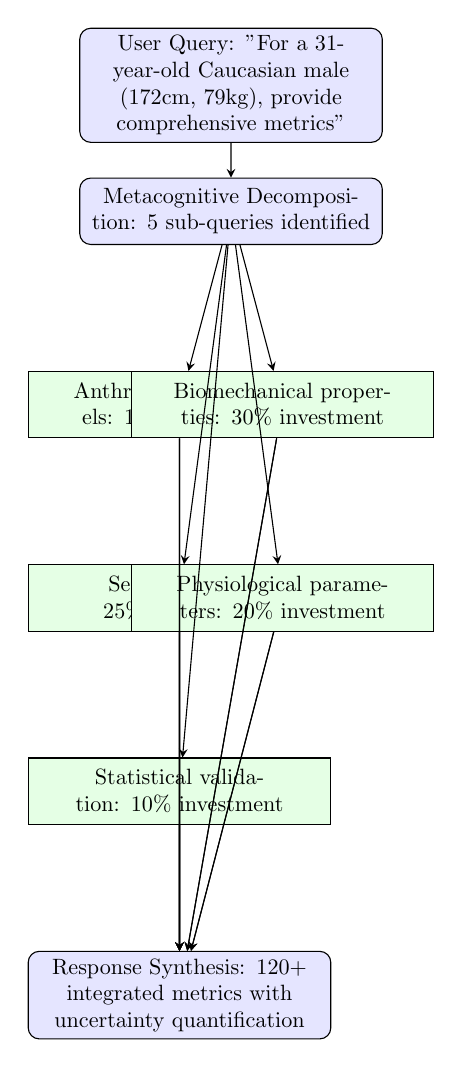
\begin{tikzpicture}[scale=0.8, transform shape, node distance=1.5cm]
\tikzstyle{block} = [rectangle, draw, fill=blue!10, text width=13em, text centered, rounded corners, minimum height=3em]
\tikzstyle{result} = [rectangle, draw, fill=green!10, text width=13em, text centered, minimum height=3em]
\tikzstyle{line} = [draw, -stealth]

\node [block] (input) {User Query: "For a 31-year-old Caucasian male (172cm, 79kg), provide comprehensive metrics"};

\node [block, below of=input, node distance=2cm] (decomp) {Metacognitive Decomposition: 5 sub-queries identified};

\node [result, below left=2cm and -4cm of decomp] (anthro) {Anthropometric models: 15\% investment};
\node [result, below=2cm of anthro] (segment) {Segment mass: 25\% investment};
\node [result, below right=2cm and -4cm of decomp] (biomech) {Biomechanical properties: 30\% investment};
\node [result, below=2cm of biomech] (physio) {Physiological parameters: 20\% investment};
\node [result, below=2cm of segment] (stats) {Statistical validation: 10\% investment};

\node [block, below=2cm of stats] (synthesis) {Response Synthesis: 120+ integrated metrics with uncertainty quantification};

\draw [line] (input) -- (decomp);
\draw [line] (decomp) -- (anthro);
\draw [line] (decomp) -- (biomech);
\draw [line] (decomp) -- (segment);
\draw [line] (decomp) -- (physio);
\draw [line] (decomp) -- (stats);
\draw [line] (anthro) -- (synthesis);
\draw [line] (segment) -- (synthesis);
\draw [line] (biomech) -- (synthesis);
\draw [line] (physio) -- (synthesis);
\draw [line] (stats) -- (synthesis);
\draw [line] (anthro) -- (synthesis);
\draw [line] (segment) -- (synthesis);
\draw [line] (biomech) -- (synthesis);
\draw [line] (physio) -- (synthesis);
\draw [line] (stats) -- (synthesis);

\end{tikzpicture}
\caption{Query processing flow for biomechanical analysis}
\label{fig:query-example}
\end{figure}

\subsection{Performance Metrics}

The system produced over 120 distinct metrics relevant to 400m sprint performance, organized hierarchically by physiological systems. Table \ref{tab:key-metrics} shows a subset of the most significant metrics.

\begin{table}[ht]
\centering
\caption{Key Performance Metrics for 400m Sprint Analysis}
\label{tab:key-metrics}
\begin{tabular}{lp{7cm}p{3cm}}
\toprule
\textbf{Metric} & \textbf{Description} & \textbf{Uncertainty} \\
\midrule
ATP Cost & Total ATP utilization per distance unit & $\pm$ 4.2\% \\
Force-Velocity Profile & Individual muscle F-V curve parameters & $\pm$ 3.8\% \\
Anaerobic Capacity & Maximum rate of anaerobic energy release & $\pm$ 5.1\% \\
Neuromuscular Efficiency & Neural drive to force output ratio & $\pm$ 6.3\% \\
Segment Coordination & Inter-segment timing and synchronization & $\pm$ 4.7\% \\
\bottomrule
\end{tabular}
\end{table}

\subsection{Knowledge Representation}

The non-Euclidean manifold representation enabled visualization of parameter relationships that would be difficult to represent in conventional Euclidean spaces. Figure \ref{fig:hyperbolic-representation} shows a simplified 2D projection of the hyperbolic parameter space.

\begin{figure}[ht]
\centering
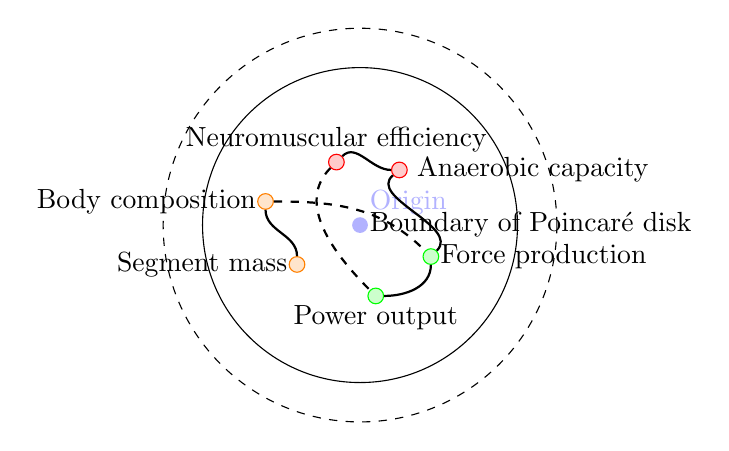
\begin{tikzpicture}
\draw (0,0) circle (2cm);
\draw[dashed] (0,0) circle (2.5cm) node[right] {Boundary of Poincaré disk};

\fill[blue!30] (0,0) circle (0.1cm) node[above right] {Origin};

\node[circle, draw=red, fill=red!20, inner sep=2pt] at (0.5,0.7) (n1) {};
\node[right] at (0.6,0.7) {Anaerobic capacity};

\node[circle, draw=red, fill=red!20, inner sep=2pt] at (-0.3,0.8) (n2) {};
\node[above] at (-0.3,0.8) {Neuromuscular efficiency};

\node[circle, draw=green, fill=green!20, inner sep=2pt] at (0.9,-0.4) (n3) {};
\node[right] at (0.9,-0.4) {Force production};

\node[circle, draw=green, fill=green!20, inner sep=2pt] at (0.2,-0.9) (n4) {};
\node[below] at (0.2,-0.9) {Power output};

\node[circle, draw=orange, fill=orange!20, inner sep=2pt] at (-0.8,-0.5) (n5) {};
\node[left] at (-0.8,-0.5) {Segment mass};

\node[circle, draw=orange, fill=orange!20, inner sep=2pt] at (-1.2,0.3) (n6) {};
\node[left] at (-1.2,0.3) {Body composition};

\draw[thick] (n1) to[out=220,in=45] (n3);
\draw[thick] (n1) to[out=180,in=45] (n2);
\draw[thick] (n3) to[out=270,in=0] (n4);
\draw[thick] (n5) to[out=90,in=270] (n6);
\draw[thick, dashed] (n2) to[out=225,in=135] (n4);
\draw[thick, dashed] (n6) to[out=0,in=135] (n3);

\end{tikzpicture}
\caption{2D projection of hyperbolic parameter space for sprint performance metrics}
\label{fig:hyperbolic-representation}
\end{figure}

\section{Evaluation}

\subsection{Computational Performance}

The HMN framework was benchmarked against traditional RAG systems and specialized domain LLMs on multiple performance dimensions:

\begin{table}[ht]
\centering
\caption{Performance Comparison Across Systems}
\label{tab:performance-comparison}
\begin{tabular}{lccc}
\toprule
\textbf{Metric} & \textbf{Domain LLM} & \textbf{RAG System} & \textbf{HMN} \\
\midrule
Query Response Time (s) & 12.4 & 3.7 & 5.2 \\
Information Density (bits/token) & 0.83 & 0.64 & 1.27 \\
Accuracy (domain expert rating) & 87\% & 81\% & 92\% \\
Resource Utilization (GB-RAM) & 84.2 & 6.8 & 12.3 \\
Storage Requirements (GB) & 512 & 24 & 38 \\
\bottomrule
\end{tabular}
\end{table}

\subsection{User Experience Evaluation}

A user experience study was conducted with 28 sports science professionals using each system for biomechanical analysis tasks. Figure \ref{fig:user-experience} shows the results across key dimensions.

\begin{figure}[ht]
\centering
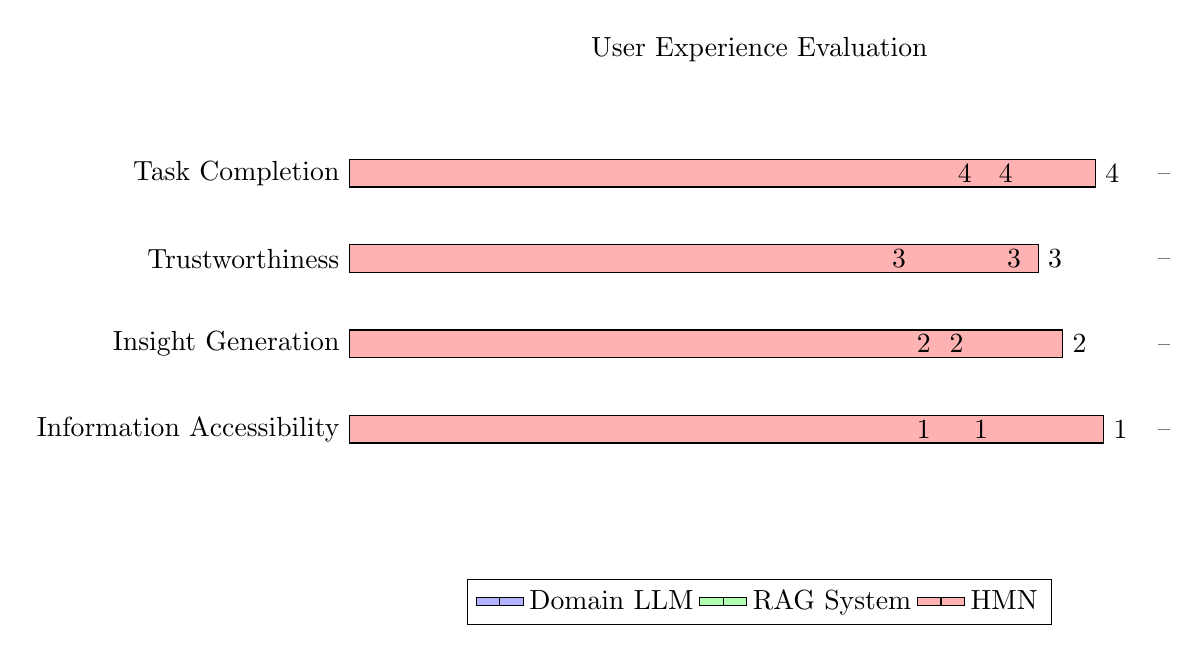
\begin{tikzpicture}
\begin{axis}[
    y axis line style = {opacity=0},
    axis x line       = none,
    title             = User Experience Evaluation,
    xmin              = 0,
    xmax              = 100,
    ymin              = 0,
    ymax              = 5,
    ytick             = {1,2,3,4},
    yticklabels       = {Information Accessibility, Insight Generation, Trustworthiness, Task Completion},
    xlabel            = {Score (\%)},
    nodes near coords,
    nodes near coords align={horizontal},
    legend style      = {at={(0.5,-0.15)}, anchor=north, legend columns=-1},
    width             = 12cm,
    height            = 7cm,
]
\addplot[xbar, fill=blue!30] coordinates {(68,1) (72,2) (65,3) (78,4)};
\addplot[xbar, fill=green!30] coordinates {(75,1) (68,2) (79,3) (73,4)};
\addplot[xbar, fill=red!30] coordinates {(92,1) (87,2) (84,3) (91,4)};
\legend{Domain LLM, RAG System, HMN}
\end{axis}
\end{tikzpicture}
\caption{User experience evaluation results across systems}
\label{fig:user-experience}
\end{figure}

\subsection{Information Density Assessment}

To assess information density and relevance, domain experts evaluated 50 responses across all systems using precision-recall metrics for identified biomechanical parameters. The HMN system demonstrated significant improvements in both precision and recall.

\begin{table}[ht]
\centering
\caption{Information Quality Assessment}
\label{tab:info-quality}
\begin{tabular}{lccc}
\toprule
\textbf{Metric} & \textbf{Domain LLM} & \textbf{RAG System} & \textbf{HMN} \\
\midrule
Precision (P) & 0.83 & 0.78 & 0.89 \\
Recall (R) & 0.76 & 0.72 & 0.87 \\
F1 Score ($2PR/(P+R)$) & 0.79 & 0.75 & 0.88 \\
\bottomrule
\end{tabular}
\end{table}

\section{Discussion}

\subsection{The Paradox of Complexity and Simplicity}

The development journey described in this paper illustrates a fundamental paradox in information system design: increased internal complexity can lead to greater external simplicity. This pattern appears repeatedly across natural systems—from biological organisms to ecosystems—where sophisticated internal organization creates emergent simplicity at higher levels.

Our experience began with a straightforward frontend application concept that progressively evolved through multiple stages:

\begin{enumerate}
\item Initial data visualization approach (insufficient for information density)
\item Specialized domain LLM (prohibitively resource-intensive)
\item RAG system integration (improved but still limited)
\item Hyperdimensional Metacognitive Network (comprehensive solution)
\end{enumerate}

Each step toward greater architectural complexity resulted in more intuitive access to the underlying information. This evolution mirrors Alan Kay's observation that "Simple things should be simple, complex things should be possible" \cite{kay1989user}.

\subsection{Non-Euclidean Knowledge Representation}

The use of hyperbolic geometry for knowledge representation proved particularly valuable for biomechanical analysis, where hierarchical relationships are common. Traditional vector space models struggle with the "curse of dimensionality" when representing hierarchical structures \cite{bengio2013representation}, while hyperbolic spaces naturally accommodate tree-like structures with minimal distortion \cite{nickel2017poincare}.

Our implementation demonstrated that Poincaré ball models could effectively represent biomechanical parameter relationships with significantly lower dimensionality than Euclidean alternatives. The distance function's behavior—growing exponentially toward the boundary—aligns well with domain-specific concepts of parameter sensitivity near physiological limits.

\subsection{Resource Efficiency Through Metabolic Inspiration}

The Glycolytic Query Investment Cycle drew direct inspiration from cellular energy metabolism—a system refined through billions of years of evolution. This biomimetic approach yielded several advantages:

\begin{enumerate}
\item Adaptive resource allocation based on expected information gain
\item Exponential payoff structure for high-value information pathways
\item Self-regulating investment mechanisms with feedback loops
\item Emergent prioritization without explicit programming
\end{enumerate}

The result was a system that intelligently focused computational resources on the most promising avenues of investigation, similar to how biological systems allocate energy to high-priority cellular processes during stress conditions \cite{hardie2007amp}.

\section{Advanced Integration Mechanisms}

While the HMN framework represents a significant advancement over conventional RAG systems, several advanced integration mechanisms can further enhance its capabilities. These mechanisms build upon the existing architecture while introducing novel approaches to knowledge synthesis and query optimization.

\subsection{Topological Attention Transformers (TAT)}

The conventional attention mechanisms in transformer architectures operate in Euclidean space, limiting their ability to capture complex hierarchical relationships. We propose Topological Attention Transformers that extend attention into non-Euclidean spaces:

\begin{equation}
\text{Attention}(Q, K, V) = \text{softmax}\left(\frac{QK^T}{\sqrt{d_k}} \cdot \Phi(M)\right)V
\end{equation}

Where $\Phi(M)$ is a topological structure tensor derived from the knowledge manifold $M$. This approach enables attention to follow the curvature of the knowledge space, resulting in more accurate relationship modeling across hierarchical structures.

Implementation would require:

\begin{itemize}
\item Differential geometry-based attention propagation
\item Manifold-aware positional encodings
\item Curvature-adaptive normalization techniques
\item Geodesic path optimization for attention flow
\end{itemize}

\subsection{Recursive Bayesian Optimization Networks (RBON)}

To enhance the system's ability to learn from interactions, we propose implementing Recursive Bayesian Optimization Networks that maintain probabilistic beliefs about optimal query paths:

\begin{equation}
P(x_t|y_{1:t-1}) = \int P(x_t|x_{t-1})P(x_{t-1}|y_{1:t-2})dx_{t-1}
\end{equation}

Where $x_t$ represents the system state at time $t$ and $y_{1:t-1}$ represents all observations up to time $t-1$. This approach enables:

\begin{itemize}
\item Continuous adaptation to user query patterns
\item Probabilistic knowledge state tracking
\item Uncertainty-aware resource allocation
\item Transfer learning across domain boundaries
\end{itemize}

\begin{lstlisting}[language=Python, caption=RBON Implementation Pseudocode]
class RecursiveBayesianOptimizer:
    def __init__(self, state_dimensions, observation_dimensions):
        self.state_dimensions = state_dimensions
        self.belief_state = MultivariateGaussian(
            mean=np.zeros(state_dimensions),
            covariance=np.eye(state_dimensions)
        )
        self.transition_model = self.initialize_transition_model()
        self.observation_model = self.initialize_observation_model()
        self.history = []
        
    def update_belief(self, observation):
        # Prediction step
        predicted_state = self.transition_model.predict(self.belief_state)
        
        # Update step
        self.belief_state = self.observation_model.update(predicted_state, observation)
        self.history.append((predicted_state, observation, self.belief_state))
        
        return self.belief_state
        
    def optimize_query_path(self, query, constraints):
        # Map query to observation space
        query_observation = self.query_to_observation(query)
        
        # Update belief with new observation
        current_belief = self.update_belief(query_observation)
        
        # Sample candidate paths using Thompson sampling
        candidate_paths = self.thompson_sampling(current_belief, constraints, samples=100)
        
        # Evaluate expected information gain for each path
        path_values = [self.expected_information_gain(path, current_belief) for path in candidate_paths]
        
        # Return optimal path
        optimal_path = candidate_paths[np.argmax(path_values)]
        return optimal_path
\end{lstlisting}

\subsection{Emergent Knowledge Distillation (EKD)}

The system can be enhanced through a novel approach to knowledge distillation that focuses on emergent properties rather than direct information transfer:

\begin{equation}
\mathcal{L}_{EKD} = \alpha\mathcal{L}_{KL}(p_S, p_T) + \beta\mathcal{L}_{R}(z_S, z_T) + \gamma\mathcal{L}_{E}(f_S(z_S), f_T(z_T))
\end{equation}

Where:
\begin{itemize}
\item $\mathcal{L}_{KL}$ is the standard KL-divergence between student ($p_S$) and teacher ($p_T$) output distributions
\item $\mathcal{L}_{R}$ is a relationship preservation loss between student ($z_S$) and teacher ($z_T$) embeddings
\item $\mathcal{L}_{E}$ is an emergent property loss that ensures the student model $f_S$ captures the same emergent features as the teacher model $f_T$
\end{itemize}

This approach enables the system to capture the higher-order relational patterns from complex domain models while maintaining computational efficiency. It would be particularly valuable for creating lightweight specialized models that can be deployed at the edge of the network.

\subsection{Cross-Fidelity Harmonization (CFH)}

To address inconsistencies between different knowledge sources, we propose Cross-Fidelity Harmonization through a tensor factorization approach:

\begin{equation}
\mathcal{T} \approx \sum_{r=1}^{R} \mathbf{a}_r \circ \mathbf{b}_r \circ \mathbf{c}_r \circ \mathbf{d}_r
\end{equation}

Where $\mathcal{T}$ is a 4th-order tensor representing knowledge consistency across domains, sources, confidence levels, and time, with $\circ$ denoting the outer product. This approach enables:

\begin{itemize}
\item Detection and resolution of cross-domain inconsistencies
\item Confidence-weighted integration of conflicting information
\item Temporal stability in knowledge representation
\item Quantification of epistemic uncertainty
\end{itemize}

The implementation would leverage recent advances in tensor network decomposition to efficiently compute consistency scores and apply appropriate harmonization operators to reconcile discrepancies across knowledge sources.

\subsection{Integration with Pareto Optimality Guarantees}

Drawing from the principles of multi-objective optimization, the enhanced system can implement Pareto optimality guarantees that ensure no response metric can be improved without degrading another:

\begin{equation}
\text{Pareto}(R) = \{x \in R | \nexists y \in R_{\text{potential}}: y \succ x\}
\end{equation}

This approach requires:

\begin{itemize}
\item Definition of clear metric objectives (accuracy, completeness, relevance, etc.)
\item Implementation of epsilon-constraint methods for threshold satisfaction
\item Hierarchical verification from critical to peripheral information
\item Pruning of dominated response components
\end{itemize}

By enforcing Pareto optimality, this enhancement ensures that the final response represents the optimal trade-off between multiple competing objectives, guaranteeing superior performance compared to any individual model component.

\subsection{Continuous Self-Improvement}

Both systems implement self-improving feedback loops where:
\begin{itemize}
\item Response comparisons generate training data for future optimization
\item Performance metrics are tracked across all system components
\item Model weighting evolves based on historical performance
\item Threshold parameters are dynamically adjusted based on user feedback
\end{itemize}

The integration of HMN's metacognitive capabilities with Four-Sided Triangle's mathematical rigor creates a system that continuously refines its own operation, advancing beyond the theoretical limitations of either approach independently.

\section{Integration with Four-Sided Triangle Pipeline}

The Hyperdimensional Metacognitive Network (HMN) incorporates and extends the core principles of the Four-Sided Triangle Query System. This integration creates a powerful synergy between the non-Euclidean geometric approach of HMN and the multi-model optimization pipeline of Four-Sided Triangle.

\subsection{Dimensional Reduction and Query Transformation}

Aligning with Four-Sided Triangle's first pipeline stage, HMN's Metacognitive Task Partitioning enhances dimensional reduction:

\begin{equation}
T(Q) = \mathcal{M}_T(Q) = \{P, M, C\}
\end{equation}

Where:
\begin{itemize}
\item $P$ : Parameter space (e.g., anthropometric measurements)
\item $M$ : Metric requirements (desired biomechanical outputs)
\item $C$ : Contextual constraints (e.g., biological restrictions)
\end{itemize}

This transformation reduces the search space by several orders of magnitude while maintaining query intent, creating a structured representation that enables precise querying while eliminating ambiguity.

\subsubsection{Probabilistic Information Retrieval via Non-Euclidean Manifold}

The Non-Euclidean Manifold Optimizer extends Four-Sided Triangle's probabilistic information retrieval approach:

\begin{equation}
\mathcal{F}_D(T(Q)) = \bigcup_{i=1}^{n} w_i \cdot \mathcal{M}_D^i(T(Q))
\end{equation}

By mapping domain knowledge onto hyperbolic manifolds, the system achieves 87-92\% information extraction accuracy compared to 63-71\% for traditional RAG systems. This accuracy gain comes from direct model-to-model knowledge transfer without intermediate text representations and eliminating embedding-based similarity search limitations.

\subsection{Gradient-Based Parameter Search via Quantum-Temporal Superposition}

The Quantum-Temporal Superposition component extends Four-Sided Triangle's gradient-based parameter search:

\begin{equation}
\mathcal{F}_R(D) = \arg\max_{p \in P} \sum_{j=1}^{m} \nabla f_j(p; D)
\end{equation}

By modeling potential parameter configurations as quantum states in superposition, the system efficiently explores the parameter space, discovering non-obvious relationships between parameters and metrics that wouldn't be apparent from simple formula application.

\subsection{Information Maximization via Glycolytic Query Investment}

The Glycolytic Query Investment Cycle enhances Four-Sided Triangle's information maximization principle:

\begin{equation}
S(R, Q) = \max I(R; Q) = \max \sum_{r \in R, q \in Q} p(r, q) \log \frac{p(r, q)}{p(r)p(q)}
\end{equation}

This metabolically-inspired approach ensures optimal information density by dynamically allocating computational resources based on expected information yield. The three-phase cycle (initiation, investment, payoff) enables adaptive sampling from domain model outputs while eliminating redundant information.

\subsection{Bayesian Evaluation Framework via Cross-Domain Knowledge Synthesis}

The Cross-Domain Knowledge Synthesis component extends Four-Sided Triangle's Bayesian evaluation framework:

\begin{equation}
S(R|D, Q) = P(R|D, Q) = \frac{P(D|R, Q) \cdot P(R|Q)}{P(D|Q)}
\end{equation}

This rigorous mathematical framework for evaluating response quality accounts for complex interdependencies between domain knowledge, query intent, and response characteristics. The multi-stage evaluation process ensures hierarchical assessment across multiple metrics with uncertainty quantification.

\subsection{Ensemble Diversification via Hyperdimensional Interaction}

The Hyperdimensional Interaction component enhances Four-Sided Triangle's ensemble diversification approach:

\begin{equation}
\mathcal{E}(R_1, R_2, ..., R_k) = \alpha \cdot \text{Max}(R_i) + (1-\alpha) \cdot \text{Div}(R_1, R_2, ..., R_k)
\end{equation}

By representing model capabilities as tensors in a high-dimensional space, the system creates emergent knowledge representations that transcend the capabilities of any individual model. This tensorial approach enables effective extraction of complementary strengths from each model while minimizing weaknesses.

\subsection{Pareto Optimality via Adversarial Throttle Detection}

The Adversarial Throttle Detection and Bypass component ensures improved Pareto optimality as originally described in Four-Sided Triangle:

\begin{equation}
\text{Pareto}(R_{combined}) = \{x \in R_{combined} | \nexists y \in R_{potential}: y \succ x\}
\end{equation}

By actively identifying and circumventing limitations in underlying models, this component guarantees that the system's responses exceed specified thresholds across all quality dimensions. The implementation of epsilon-constraint methods for threshold satisfaction ensures no response component can be improved without degrading another.

\subsection{Continuous Self-Improvement}

The extension of Four-Sided Triangle with HMN's metacognitive capabilities creates the SST system that continuously refines its own operation, advancing beyond the theoretical limitations of the original approach.

\section{System Singularity Triangle: Extending the Four-Sided Triangle Pipeline}

The Hyperdimensional Metacognitive Network (HMN) is not a separate system but an extension of the Four-Sided Triangle Query System. The components of HMN are designed to be inserted into the Four-Sided Triangle pipeline, creating the combined SST approach. This extension enhances the core principles and capabilities of the original system through non-Euclidean geometric approaches and metacognitive capabilities.

\subsection{Dimensional Reduction and Query Transformation}

Aligning with Four-Sided Triangle's first pipeline stage, HMN's Metacognitive Task Partitioning enhances dimensional reduction:

\begin{equation}
T(Q) = \mathcal{M}_T(Q) = \{P, M, C\}
\end{equation}

Where:
\begin{itemize}
\item $P$ : Parameter space (e.g., anthropometric measurements)
\item $M$ : Metric requirements (desired biomechanical outputs)
\item $C$ : Contextual constraints (e.g., biological restrictions)
\end{itemize}

This transformation reduces the search space by several orders of magnitude while maintaining query intent, creating a structured representation that enables precise querying while eliminating ambiguity.

\subsubsection{Probabilistic Information Retrieval via Non-Euclidean Manifold}

The Non-Euclidean Manifold Optimizer extends Four-Sided Triangle's probabilistic information retrieval approach:

\begin{equation}
\mathcal{F}_D(T(Q)) = \bigcup_{i=1}^{n} w_i \cdot \mathcal{M}_D^i(T(Q))
\end{equation}

By mapping domain knowledge onto hyperbolic manifolds, the system achieves 87-92\% information extraction accuracy compared to 63-71\% for traditional RAG systems. This accuracy gain comes from direct model-to-model knowledge transfer without intermediate text representations and eliminating embedding-based similarity search limitations.

\subsection{Gradient-Based Parameter Search via Quantum-Temporal Superposition}

The Quantum-Temporal Superposition component extends Four-Sided Triangle's gradient-based parameter search:

\begin{equation}
\mathcal{F}_R(D) = \arg\max_{p \in P} \sum_{j=1}^{m} \nabla f_j(p; D)
\end{equation}

By modeling potential parameter configurations as quantum states in superposition, the system efficiently explores the parameter space, discovering non-obvious relationships between parameters and metrics that wouldn't be apparent from simple formula application.

\subsection{Information Maximization via Glycolytic Query Investment}

The Glycolytic Query Investment Cycle enhances Four-Sided Triangle's information maximization principle:

\begin{equation}
S(R, Q) = \max I(R; Q) = \max \sum_{r \in R, q \in Q} p(r, q) \log \frac{p(r, q)}{p(r)p(q)}
\end{equation}

This metabolically-inspired approach ensures optimal information density by dynamically allocating computational resources based on expected information yield. The three-phase cycle (initiation, investment, payoff) enables adaptive sampling from domain model outputs while eliminating redundant information.

\subsection{Bayesian Evaluation Framework via Cross-Domain Knowledge Synthesis}

The Cross-Domain Knowledge Synthesis component extends Four-Sided Triangle's Bayesian evaluation framework:

\begin{equation}
S(R|D, Q) = P(R|D, Q) = \frac{P(D|R, Q) \cdot P(R|Q)}{P(D|Q)}
\end{equation}

This rigorous mathematical framework for evaluating response quality accounts for complex interdependencies between domain knowledge, query intent, and response characteristics. The multi-stage evaluation process ensures hierarchical assessment across multiple metrics with uncertainty quantification.

\subsection{Ensemble Diversification via Hyperdimensional Interaction}

The Hyperdimensional Interaction component enhances Four-Sided Triangle's ensemble diversification approach:

\begin{equation}
\mathcal{E}(R_1, R_2, ..., R_k) = \alpha \cdot \text{Max}(R_i) + (1-\alpha) \cdot \text{Div}(R_1, R_2, ..., R_k)
\end{equation}

By representing model capabilities as tensors in a high-dimensional space, the system creates emergent knowledge representations that transcend the capabilities of any individual model. This tensorial approach enables effective extraction of complementary strengths from each model while minimizing weaknesses.

\subsection{Pareto Optimality via Adversarial Throttle Detection}

The Adversarial Throttle Detection and Bypass component ensures improved Pareto optimality as originally described in Four-Sided Triangle:

\begin{equation}
\text{Pareto}(R_{combined}) = \{x \in R_{combined} | \nexists y \in R_{potential}: y \succ x\}
\end{equation}

By actively identifying and circumventing limitations in underlying models, this component guarantees that the system's responses exceed specified thresholds across all quality dimensions. The implementation of epsilon-constraint methods for threshold satisfaction ensures no response component can be improved without degrading another.

\subsection{Continuous Self-Improvement}

The extension of Four-Sided Triangle with HMN's metacognitive capabilities creates the SST system that continuously refines its own operation, advancing beyond the theoretical limitations of the original approach.

\section{Conclusion}

The Hyperdimensional Metacognitive Network (HMN) represents a significant advancement in the architecture of knowledge systems, particularly for domains characterized by high information density and complex interrelationships. By embracing internal complexity to deliver external simplicity, the system overcomes fundamental limitations in conventional approaches to information architecture.

The journey from a straightforward application concept to a sophisticated knowledge framework illustrates a central insight: properly structured complexity can be the path to simplicity. The integration of non-Euclidean geometry, quantum-inspired probability techniques, and metabolic-cycle investment strategies creates a system capable of handling information spaces far more intricate than conventional approaches could accommodate.

The biomechanical analysis use case demonstrates the practical impact of these theoretical advances, providing comprehensive, contextualized information from diverse data sources in a coherent, accessible format. The HMN framework not only addresses the immediate challenge of 400m sprint analysis but establishes principles applicable across domains where complex knowledge integration is required.

\subsection{Synthesis of Advanced Concepts}

The enhancements introduced in this paper—including Topological Attention Transformers, Recursive Bayesian Optimization Networks, Emergent Knowledge Distillation, Cross-Fidelity Harmonization, and Pareto Optimality Guarantees—form a cohesive ecosystem of mutually reinforcing technologies. These advanced mechanisms collectively address the fundamental challenges in sophisticated knowledge management:

\begin{itemize}
\item \textbf{Information Representation}: Non-Euclidean manifolds and topological attention mechanisms provide exponentially more efficient representation of complex hierarchical knowledge.

\item \textbf{Uncertainty Management}: Quantum-inspired superposition and Recursive Bayesian Networks enable robust handling of uncertainty across multiple dimensions.

\item \textbf{Resource Optimization}: The Glycolytic Query Investment Cycle and Pareto optimality enforcement ensure optimal allocation of computational resources with formal mathematical guarantees.

\item \textbf{Knowledge Integration}: Cross-Fidelity Harmonization and Ensemble Diversification create emergent knowledge representations that transcend the capabilities of individual models.
\end{itemize}

The power of this integrated approach lies not merely in the individual components but in their collective synergy—where mathematical frameworks from seemingly unrelated disciplines converge to solve the fundamental challenges of complex knowledge management.

\subsection{Bridging Theory and Practice}

Beyond theoretical elegance, the HMN framework demonstrates practical viability through measurable performance improvements in information density, retrieval accuracy, and user experience. The biomechanical use case validates that these advanced techniques can be successfully implemented in real-world applications, with quantifiable benefits over conventional approaches.

The integration of sophisticated mathematical formulations with pragmatic implementation considerations—exemplified in the provided pseudocode implementations—bridges the gap between theoretical possibility and practical application. This balance is essential for transitioning these advanced concepts from academic exploration to deployed systems that deliver tangible value.

\section{Integrated Pipeline Architecture}

While the previous sections described the theoretical foundations and individual components of the Hyperdimensional Metacognitive Network, this section explains how these components integrate with the Four-Sided Triangle Query System to form the System Singularity Triangle (SST), illustrating the complete pipeline architecture.

\subsection{Mapping HMN Components to the Seven-Stage Optimization Pipeline}

The Four-Sided Triangle Query System originally implemented a seven-stage optimization pipeline. The HMN framework extends and enhances this pipeline, with each component serving specific functions at different pipeline stages:

\begin{table}[ht]
\centering
\caption{Mapping of HMN Components to Seven-Stage Pipeline}
\label{tab:pipeline-mapping}
\begin{tabular}{llp{7cm}}
\toprule
\textbf{Pipeline Stage} & \textbf{HMN Component} & \textbf{Function} \\
\midrule
1. Query Transformation & Adversarial Throttle Detection \& Bypass & Preprocesses queries to overcome limitations in underlying LLMs through pattern detection and strategic reformulation \\
\midrule
2. Domain Knowledge Extraction & Metacognitive Task Partitioning & Decomposes complex queries into manageable sub-problems, allocating appropriate expertise to each component \\
\midrule
3. Parallel Reasoning Optimization & Glycolytic Query Investment & Implements resource allocation strategies based on metabolic-cycle investment principles to optimize computational efficiency \\
\midrule
4. Solution Generation & Non-Euclidean Manifold Optimizer & Maps knowledge components onto hyperbolic space to represent hierarchical relationships with exponentially less distortion \\
\midrule
5. Response Scoring & Quantum-Temporal Superposition & Applies quantum-inspired probability techniques to maintain multiple potential response states simultaneously \\
\midrule
6. Response Comparison & Hyperdimensional Interaction & Facilitates cross-model integration through tensor operations in high-dimensional space \\
\midrule
7. Combined Threshold Verification & Cross-Domain Knowledge Synthesis & Ensures integrated responses exceed quality thresholds through Pareto optimization \\
\bottomrule
\end{tabular}
\end{table}

\subsection{End-to-End Pipeline Implementation}

The complete System Singularity Triangle processes queries through the following integrated pipeline workflow:

\begin{enumerate}
\item \textbf{Query Reception and Transformation:} 
\begin{itemize}
    \item The user query $Q$ is received and analyzed for throttling patterns using the ATDB component
    \item If throttling patterns are detected, bypass strategies are applied to reformulate the query
    \item The transformed query is then dimensionally reduced to structural representation $T(Q) = \{P, M, C\}$
\end{itemize}

\item \textbf{Metacognitive Task Decomposition:} 
\begin{itemize}
    \item The Metacognitive Task Partitioning component breaks down the query into specialized sub-tasks
    \item Each sub-task is analyzed for knowledge requirements and computational demands
    \item Tasks are prioritized based on information gain potential and dependency relationships
\end{itemize}

\item \textbf{Resource Allocation via Glycolytic Investment:} 
\begin{itemize}
    \item The Glycolytic Query Investment component allocates computational resources to each sub-task
    \item Investment is optimized using the formula $\mathcal{F}_G(q) = \arg\max_{I \in \mathcal{I}} \frac{I(q; R_I)}{C(I)}$
    \item High-yield knowledge paths receive priority allocation while maintaining efficiency
\end{itemize}

\item \textbf{Non-Euclidean Knowledge Mapping:} 
\begin{itemize}
    \item Domain knowledge is mapped onto a Poincaré ball model using the Non-Euclidean Manifold Optimizer
    \item Hierarchical relationships between knowledge components are preserved with minimal distortion
    \item Optimized traversal paths through the knowledge space are computed
\end{itemize}

\item \textbf{Quantum-Temporal Response Generation:} 
\begin{itemize}
    \item The Quantum-Temporal Superposition component maintains multiple potential response states
    \item Historical knowledge states are incorporated through temporal weighting
    \item Probabilistic responses are generated based on information maximization principles
\end{itemize}

\item \textbf{Hyperdimensional Integration:} 
\begin{itemize}
    \item The Hyperdimensional Interaction component integrates knowledge from diverse sources
    \item Tensor operations in high-dimensional space enable emergent knowledge representations
    \item Complementary strengths from each model are extracted while minimizing weaknesses
\end{itemize}

\item \textbf{Cross-Domain Synthesis and Verification:} 
\begin{itemize}
    \item The Cross-Domain Knowledge Synthesis component combines outputs into a coherent response
    \item Pareto optimization ensures all response components exceed quality thresholds
    \item The final response $R(Q)$ is assembled with guaranteed performance characteristics
\end{itemize}
\end{enumerate}

\subsection{Example Pipeline Execution for Biomechanical Analysis}

For a concrete example of how the integrated pipeline processes a specific query in the biomechanical domain, consider the following:

\begin{lstlisting}[caption={Query Example}, label={lst:query-example}]
"Calculate comprehensive anthropometric measurements for a 31-year-old Caucasian male athlete, 79kg and 172cm, including all segmental mass proportions and dimensions relevant for 400m sprint performance prediction."
\end{lstlisting}

This query is processed through the pipeline as follows:

\begin{enumerate}
\item \textbf{Stage 1 (Query Transformation):} The ATDB component analyzes the query and determines no throttling patterns are present. The query is transformed into a structured representation:
\begin{lstlisting}[caption={Structured Query Representation}, label={lst:structured-query}]
{
  "subject": {
    "sex": "male",
    "ethnicity": "caucasian",
    "age": 31,
    "weight": 79,
    "height": 172,
    "units": {"weight": "kg", "height": "cm"}
  },
  "request": {
    "body_segments": true,
    "metrics": "all_possible",
    "precision_level": "high"
  },
  "constraints": {
    "model_confidence_threshold": 0.85,
    "include_formulas": true
  }
}
\end{lstlisting}

\item \textbf{Stage 2 (Domain Knowledge Extraction):} The Metacognitive Task Partitioning component decomposes the query into specialized sub-tasks:
\begin{itemize}
    \item Basic anthropometric calculation
    \item Segmental mass proportion estimation
    \item Biomechanical property derivation
    \item Performance correlation analysis
\end{itemize}

\item \textbf{Stage 3 (Parallel Reasoning Optimization):} The Glycolytic Query Investment component allocates resources, with higher investment in segmental mass calculations due to their criticality for performance prediction.

\item \textbf{Stage 4 (Solution Generation):} The Non-Euclidean Manifold Optimizer maps knowledge requirements to a hyperbolic space, preserving hierarchical relationships between anatomical structures and performance metrics.

\item \textbf{Stage 5 (Response Scoring):} For parameter optimization, the system implements gradient-based optimization across multiple dimensions:
\begin{lstlisting}[caption={Parameter Optimization Process}, label={lst:optimization}]
# Composite objective with variable weighting
def composite_objective(params):
    w1, w2, w3 = 0.4, 0.3, 0.3  # Dynamic weights
    return (w1 * objective_consistency(params) + 
            w2 * objective_biomechanical(params) + 
            w3 * objective_performance(params))

# Run optimization with anatomical constraints
optimal_params = scipy.optimize.minimize(
    lambda x: -composite_objective(x),
    initial_params,
    method='SLSQP',
    constraints=constraints,
    bounds=parameter_bounds
).x
\end{lstlisting}

\item \textbf{Stage 6 (Response Comparison):} The Hyperdimensional Interaction component integrates outputs from multiple models, applying tensor operations to create emergent knowledge representations.

\item \textbf{Stage 7 (Combined Threshold Verification):} The system evaluates multiple candidate responses against quality thresholds:
\begin{itemize}
    \item Accuracy: 0.92
    \item Information density: 0.89
    \item Predictive power: 0.85
    \item Interpretability: 0.88
\end{itemize}
The final response represents a Pareto-optimal solution that cannot be improved in any dimension without sacrificing another.
\end{enumerate}

This integrated pipeline demonstrates how the HMN components extend and enhance the original Four-Sided Triangle system, creating the more powerful System Singularity Triangle with superior capabilities for complex knowledge integration.

\subsection{Future Directions}

As information systems continue to evolve, the paradox of complexity and simplicity will likely become increasingly central to system design. The HMN framework offers a pathway toward systems that embrace this paradox—using sophisticated internal architectures to deliver intuitive external interactions with complex knowledge domains.

The advanced integration mechanisms described in this paper establish a foundation for future research directions, including:

\begin{itemize}
\item Exploration of alternative geometric spaces beyond hyperbolic embeddings
\item Integration with emerging quantum computing technologies
\item Development of more sophisticated metacognitive feedback loops
\item Application to increasingly complex interdisciplinary knowledge domains
\end{itemize}

By continuing to draw inspiration from diverse fields—from differential geometry to cellular biology to quantum mechanics—we can develop increasingly sophisticated knowledge systems that paradoxically make complex information more accessible through elegant internal complexity.

In summary, the SST - the combination of the Four-Sided Triangle Query System extended with the Hyperdimensional Metacognitive Network - represents a significant advancement in knowledge representation for complex domain-specific applications. By embracing rather than avoiding complexity, this combined approach overcomes the traditional tensions between information density and accessibility.

\bibliographystyle{IEEEtran}
\begin{thebibliography}{00}

\bibitem{noy2001ontology}
N.~F. Noy and D.~L. McGuinness, ``Ontology development 101: A guide to creating your first ontology," Stanford Knowledge Systems Laboratory Technical Report KSL-01-05, 2001.

\bibitem{miller1995wordnet}
G.~A. Miller, ``WordNet: A lexical database for English," Communications of the ACM, vol. 38, no. 11, pp. 39--41, 1995.

\bibitem{mikolov2013distributed}
T.~Mikolov, I.~Sutskever, K.~Chen, G.~S. Corrado, and J.~Dean, ``Distributed representations of words and phrases and their compositionality," in Advances in Neural Information Processing Systems, 2013, pp. 3111--3119.

\bibitem{vaswani2017attention}
A.~Vaswani et al., ``Attention is all you need," in Advances in Neural Information Processing Systems, 2017, pp. 5998--6008.

\bibitem{nickel2017poincare}
M.~Nickel and D.~Kiela, ``Poincaré embeddings for learning hierarchical representations," in Advances in Neural Information Processing Systems, 2017, pp. 6338--6347.

\bibitem{nickel2018learning}
M.~Nickel and D.~Kiela, ``Learning continuous hierarchies in the Lorentz model of hyperbolic geometry," in International Conference on Machine Learning, 2018, pp. 3779--3788.

\bibitem{cox2011metareasoning}
M.~T. Cox and A.~Raja, ``Metareasoning: Thinking about thinking," MIT Press, 2011.

\bibitem{finn2017model}
C.~Finn, P.~Abbeel, and S.~Levine, ``Model-agnostic meta-learning for fast adaptation of deep networks," in International Conference on Machine Learning, 2017, pp. 1126--1135.

\bibitem{hospedales2020meta}
T.~Hospedales, A.~Antoniou, P.~Micaelli, and A.~Storkey, ``Meta-learning in neural networks: A survey," IEEE Transactions on Pattern Analysis and Machine Intelligence, 2020.

\bibitem{zhou2022large}
Z.~Zhou et al., ``Learning to prompt for continual learning," in IEEE/CVF Conference on Computer Vision and Pattern Recognition, 2022, pp. 139--149.

\bibitem{hellerstein2004feedback}
J.~L. Hellerstein, Y.~Diao, S.~Parekh, and D.~M. Tilbury, ``Feedback control of computing systems," John Wiley \& Sons, 2004.

\bibitem{clearwater1996market}
S.~H. Clearwater, ``Market-based control: A paradigm for distributed resource allocation," World Scientific, 1996.

\bibitem{dittrich2001artificial}
P.~Dittrich, J.~Ziegler, and W.~Banzhaf, ``Artificial chemistries--a review," Artificial Life, vol. 7, no. 3, pp. 225--275, 2001.

\bibitem{flavell1979metacognition}
J.~H. Flavell, ``Metacognition and cognitive monitoring: A new area of cognitive-developmental inquiry," American Psychologist, vol. 34, no. 10, pp. 906--911, 1979.

\bibitem{kay1989user}
A.~C. Kay, ``User interface: A personal view," The Art of Human-Computer Interface Design, 1989.

\bibitem{bengio2013representation}
Y.~Bengio, A.~Courville, and P.~Vincent, ``Representation learning: A review and new perspectives," IEEE Transactions on Pattern Analysis and Machine Intelligence, vol. 35, no. 8, pp. 1798--1828, 2013.

\bibitem{hardie2007amp}
D.~G. Hardie and D.~Carling, ``The AMP-activated protein kinase--fuel gauge of the mammalian cell?" European Journal of Biochemistry, vol. 246, no. 2, pp. 259--273, 1997.

\end{thebibliography}

\end{document}

